\documentclass[pdftex,12pt,a4paper]{article}

\usepackage{wrapfig, amssymb, amsmath, graphicx, subfigure, tikz}
\usepackage[dutch]{babel}
\usepackage[top=0.5in, bottom=0.5in, left=1in, right=1in]{geometry}
\usepackage{minted}
\usepackage{tabularx}
\usepackage{colortbl}
\usepackage{hhline}
\usepackage{hyperref}

\pagenumbering{arabic}
\newcommand{\HRule}{\rule{\linewidth}{0.5mm}}

\begin{document}
\begin{titlepage}

% Upper part of the page
\begin{flushleft}

\includegraphics[trim=23mm 0mm 0mm 0mm, width=1\textwidth]{./logo.jpg}\\[1cm] \end{flushleft}
\begin{center}
	\textsc{\Large Kansrekening en Statistiek}\\[0.5cm]

    % Title
    \HRule \\[0.4cm] { \huge \bfseries LAB-2}\\[0.4cm]

    \HRule \\[1.5cm]

    % Author and supervisor
\begin{minipage}{0.4\textwidth}
\begin{flushleft} \large \emph{Authors:}\\
Abe \textsc{Wiersma}\\
Stein \textsc{van Zwoll}\\
\end{flushleft}
\end{minipage}
\begin{minipage}{0.4\textwidth} \begin{flushright} \large \end{flushright}\end{minipage}

    \vfill

    % Bottom of the page 
    {\large \today}

\end{center}
\end{titlepage}
\pagebreak
\section{Deel 1}
\begin{enumerate}
    \item
        \begin{enumerate}
            \item
            	$$ f(x) =    \left\{
                                \begin{matrix}
                                    1/7 & \text{Wanneer x binnen de verdeling.}\\
                                    0 & \text{Wanneer daarbuiten.}
                                \end{matrix}
                            \right. $$
                En dus\\
                $$ F(x) =    \left\{
                                \begin{matrix}
                                    0 & \text{als $x < a$}\\
                                    (x-3)/(9-3) & \text{Wanneer x binnen de verdeling.}\\
                                    1 & \text{als $x \geq b$}
                                \end{matrix}
                            \right. $$
            \item
                $[-10,-9,...,3] \vee [3,4,...,9] = [3]$
                $P(3) = 1/7$
            \item
                $((b-a) + 1) * 1/7$
        \end{enumerate}

    \item
    	Ik had laatst nog een artikel gelezen over dat een munt niet geladen kan zijn, heeft wel aansluiting op dit
    	vraagstuk.Wel leuk.\\
    	\url{http://www.stat.columbia.edu/~gelman/research/published/diceRev2.pdf}
        \begin{enumerate}
            \item
                $U=\{kop, munt\}$
            \item
                ${n \choose k} p^k(1-p)^{n-k}$
            \item
            	De Binomiale verdeling
            \item
            	Implementatie:\\
            	\inputminted{python}{2.2d.py}
        \end{enumerate}
   	\newpage
	\item
    	Implementatie:
    	\inputminted{python}{3.py}
    	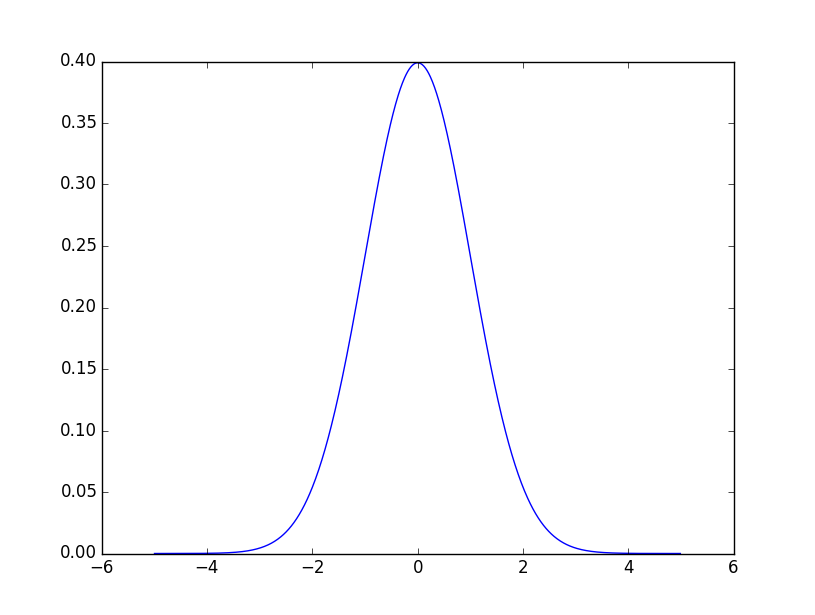
\includegraphics[width=\linewidth]{3}
    	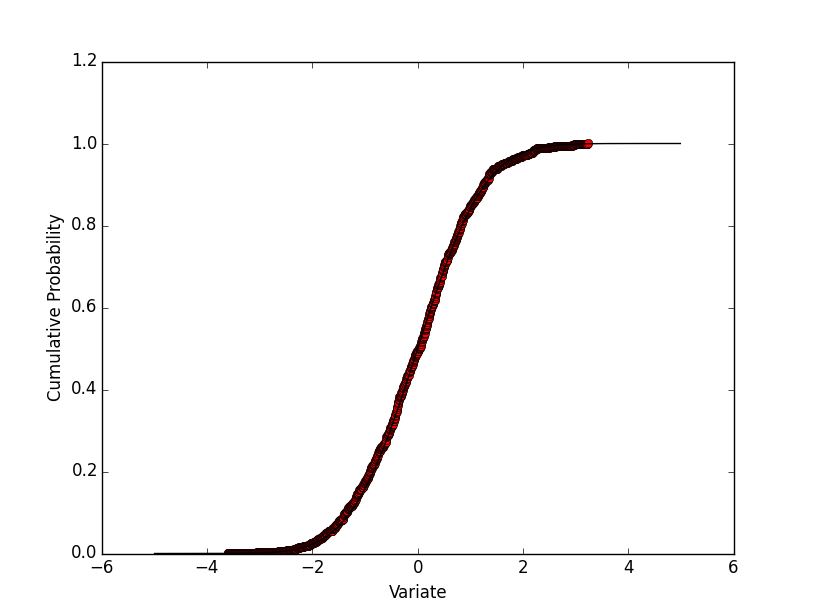
\includegraphics[width=\linewidth]{3_cum}
\end{enumerate}

\section{Naive Bayes Classifier}
	\subsection{Implementatie}
    	My python implementation:\\
    	\inputminted{python}{NaiveBayes.py}
    \subsection{Theorie}
    	Naive Bayes is a conditional probabilistic model that classifies a
    	vector to a class space. Given a vector $\mathbf{x}$ with properties
    	$x_1...x_n$, it determines the probabilities of belonging to predefined 
    	classes.In our case we have the Female Class and the Male Class.
    	And we want to check whether the probability of belonging to one class
    	is higher than belonging to the other class.\\
    	$x \in Female$ if($p(Female \vert x_1, \dots, x_n)\, > p(Male \vert x_1, \dots, x_n)\,$)\\
    	or\\
    	$x \in Male$ if($p(Male \vert x_1, \dots, x_n)\, > p(Female \vert x_1, \dots, x_n)\,$)\\
    	Using Bayes theorem this probability can then be rewritten:\\
    	$$ p((Fe)Male \vert \mathbf{x}) = \frac{p((Fe)Male) \ p(\mathbf{x} \vert
    	(Fe)Male)}{p(\mathbf{x})}. \,$$\\
    	Because the denominator is a constant in both sides of the equation it
    	can be discarded.\\
    	$$p((Fe)Male) \ p(\mathbf{x} \vert (Fe)Male) > p((Fe)Male) \
    	p(\mathbf{x} \vert (Fe)Male)$$
    	The probability to draw either a man of a woman from the population in
    	our case is also equal and can therefore also be discarded.\\
    	$$p(\mathbf{x} \vert (Fe)Male) > p(\mathbf{x} \vert (Fe)Male)$$\\
    	Here the naïvety of the classifier comes around, from here on out we
    	assume that every property of x are conditionally independent. This
    	means we can unbind $\mathbf{x}$ into it's properties:\\
    	$$p(x_{weight} \vert (Fe)Male)p(x_{length} \vert (Fe)Male)
    	p(x_{shoe\_size} \vert (Fe)Male)$$\\
    	
    	In our case as seen in my implementation we calculate the probability of a property of 
    	x within the class Male of Female by taking the Normal probability density function 
    	using the data from the database: \textrm{biometrie2014.csv}\\
    	The implementation for the classifier can be found in the $male\_or\_female$ function.
		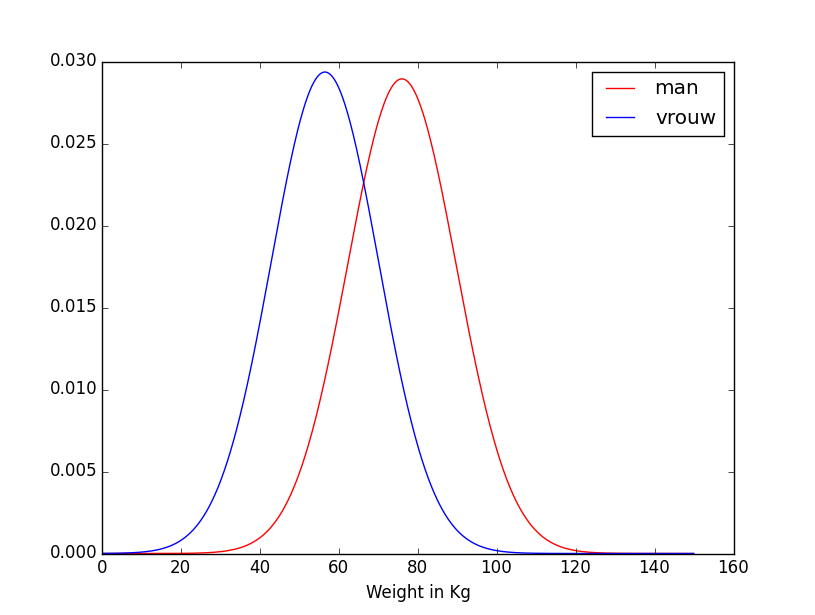
\includegraphics[width=\linewidth]{naive_weight.png}
		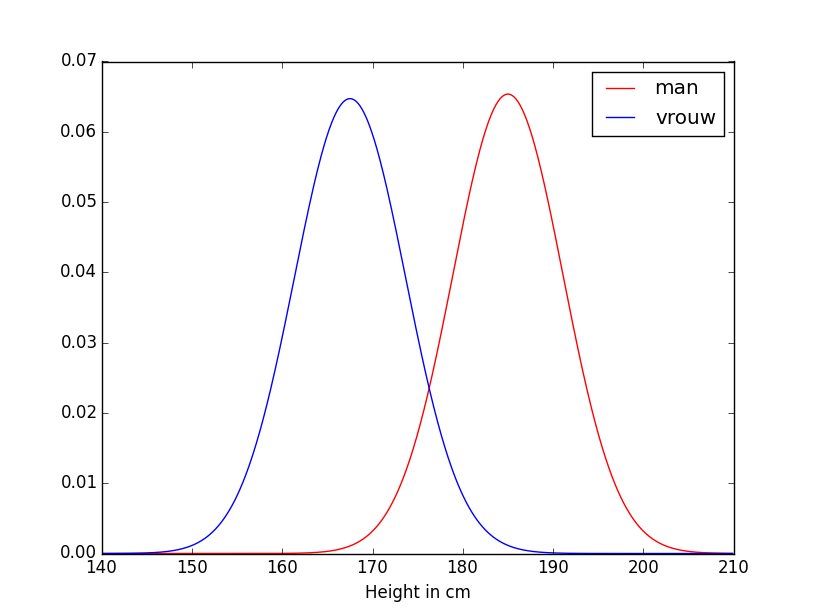
\includegraphics[width=\linewidth]{naive_height.png}
		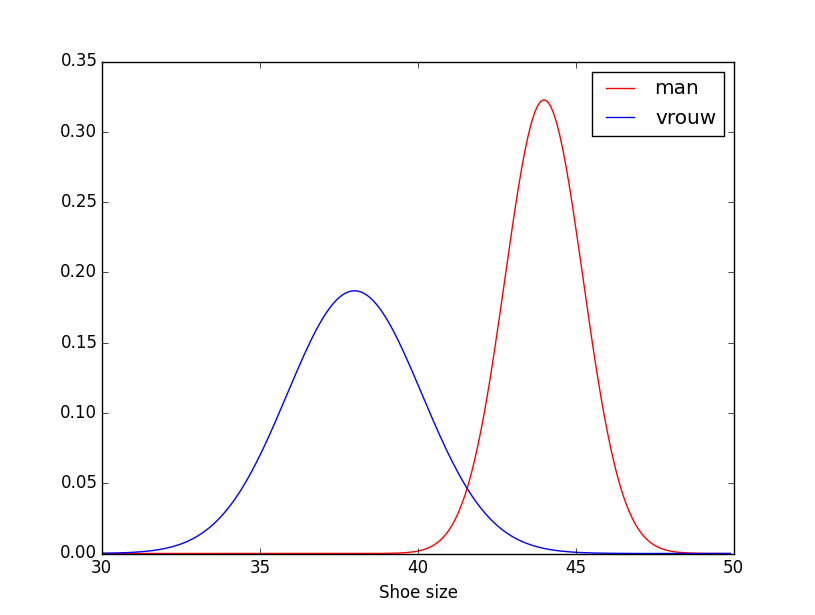
\includegraphics[width=\linewidth]{naive_shoe.png}
    	As you can see I tested using the first entry in the database, which correctly identifies as male.
    	
    	Then i check every entry in the database for class and see we come out pretty okay.
    	\begin{center}
  			\begin{tabular}{l | c | r | }
    			  & M  & F \\ \hline
    			M & 26 & 1 \\ \hline
    			F & 1  & 5 \\
    			\hline
  			\end{tabular}
		\end{center}
    	
    	
\end{document}
